\textbf{ID:} UC11 (Edit Post) \\
\textbf{Scope:} CS Automated Information Timeline \\
\textbf{Level:} User goal \\
\textbf{Primary Actor:} Faculty or Admin/Reviewer \\
\textbf{Stakeholders and Interests:}
\begin{itemize}
    \item Audience: A person that is interested in viewing all approved content on the system using their mobile device.
    \item Faculty: A person that works for the university and is interested in gaining visibility of their post and/or event.
    \item Office Manager: A person that works for the university and is interested in prioritizing the order of posts and/or events.
    \item Admin/Reviewer: A person that works for the university and approves and/or removes posts and/or events from the system.
\end{itemize}
\textbf{Preconditions:}
\begin{itemize}
    \item Faculty has been identified and authenticated.
    \item A post has been created.
\end{itemize}
\textbf{Postconditions:}
\begin{itemize}
    \item Post has been updated and saved to database.
    \item Media library has been updated with new images and videos from the updated post.
    \item The display board reflects the updated post flagged for display.
\end{itemize}
\textbf{Main Success Scenario:}
\begin{enumerate}
    \item User selects a post to edit
    \item System opens the editable view for the selected post with options to edit the text, delete the photos and videos, if present, on the post, upload photos and videos on the post and update the display flag.
    \item User saves the updated post.
    \item System presents the confirmation that the post is updated
\end{enumerate}
\textbf{Alternative Flows:}  \\
a. At any time, system fails or becomes unresponsive and does not provide an error message
\begin{enumerate}
    \item User performs a hard refresh on the browser (ctrl + f5 or shift + reload)
    \item System reloads the editable view for the post
\end{enumerate}
b. (3.a) Uploaded media is in unsupported format or exceeds the file size limit
\begin{enumerate}
    \item System prompts the user with the appropriate error message
    \item User acknowledges the error and reuploads the media in supported format and size.
\end{enumerate}

\begin{figure}[H]
    \centering
    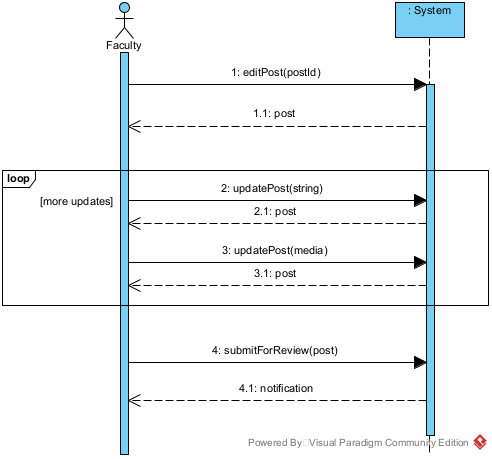
\includegraphics[width=0.8\textwidth]{images/SSD-UC11-EditPost.png}
    \centering
    \caption{System Sequence Diagram: Edit Post}
\end{figure}

\textbf{Operation:} updatePost(post) \\
\textbf{Cross Reference:} UC11 (Edit Post) \\
\textbf{Preconditions: }
\begin{itemize}
    \item Faculty has been identified and authenticated.
    \item A post has been created and persisted in the database.
    \item Update operation is underway.
\end{itemize}
\textbf{Postconditions:}
\begin{itemize}
    \item A Post instance, post was created
    \item post was associated with the Update operation.
    \item post was modified
    \item Modified post was persisted to the database
\end{itemize}